%----------------------------------------------------------
\def\notedate{2021.11.14}
\def\currentauthor{Муха В. (РК6-73Б)}
%----------------------------------------------------------
\notestatement{rndhpcedt}{Первичный обзор литературы}

%----------------------------------------------------------
\subsubsection{Известные алгоритмы поиска циклов в ориентированных графах}

Существует несколько групп алгоритмов поиска\cite{davidrajuh2016}:
\begin{enumerate}[label=\arabic*)]
    \item алгоритмы, основанные на обходе ориентированного графа (ОГ);
    \item алгоритмы, основанные на использовании матриц смежности, описывающих конкретный граф.
\end{enumerate}

Одним из представителей алгоритмов первой группы (обхода ОГ) является алгоритм поиска в глубину (англ., depth-first-search (DFS)), который предполагает, что обход осуществляется из фиксированного и заранее заданного узла. Если число узлов ОГ равно $n$, то сложность алгоритма DFS $O(n^2)$ и $O(n^3)$ -- для случая ``многократного обхода'' из каждого узла\footnote{Для случая ОГ возможность идентификации всех циклов требует осуществления многократных обходов, начиная с каждого из узлов ОГ.}. Поэтому для ускорения алгоритма необходимо применение модификаций, например распараллеливание алгоритма поиска в глубину~\cite{Mahdi2011}.

%Предполагая далее, что $n$ число узлов, з
Зададим граф $G(V, E)$, где $V = \{\bs{a}, \bs{b}, \bs{c}, \ldots\}$ -- множество вершин, $|V|=n$, а $E = \{\alpha\beta: \alpha\beta\in V\times V\}$ -- множество рёбер (пример, $\{\bs{ab}, \bs{ad}, \ldots , \bs{ge}\}$).

Для определения ОГ, часто, применяют понятие матриц смежности\cite{UUU}:\pdfcomment{Желательна ссылка на книгу о теории графов.}
\begin{equation}\label{eq.rndhpcedt.2021.11.14.01}
\begin{array}{l}
||A||=||a_{ij}||_{n\times n};\\
a_{ij}=\left\{\begin{array}{l} 1, \mbox{ -- определено ребро с началом в узле $i$ и концом в узле $j$};\\ 0, \mbox{ -- ребро не определено}.\end{array} \right.
\end{array}
\end{equation}

Пример некоторого графа и ему соответствующая матрица смежности приведены на рис.~\ref{fig.rndhpcedt.2021.11.14.01}.

\begin{figure}[!ht]
	\centering
	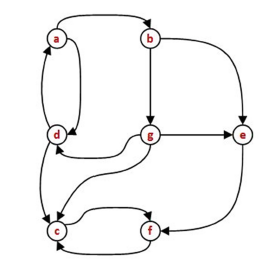
\includegraphics[width=0.3\textwidth]{ResearchNotes/rndhpc_not_edt_2021_11_14/adj_matrix.png}
	\caption{Граф и его матрица смежности}\label{fig.rndhpcedt.2021.11.14.01}
\end{figure}


\begin{equation}\label{eq.rndhpcedt.2021.11.14.00}
A=%
\begin{bmatrix}
	&	\bs{a}	&	\bs{b}	&	\bs{c}	&	\bs{d}	&	\bs{e}	&	\bs{f}	&	\bs{g} \\
\bs{a}	&	0	&	1	&	0	& 1	& 0	& 0 & 0 \\
\bs{b}	&	0	&	0	&	0	& 0	& 1	& 0 & 1 \\
\bs{c}	&	0	&	0	&	0	& 0	& 0	& 0 & 0 \\
\bs{d}	&	0	&	0	&	0	& 0	& 0	& 0 & 0 \\
\bs{e}	&	0	&	0	&	0	& 0	& 0	& 0 & 0 \\
\bs{f}	&	0	&	0	&	0	& 0	& 0	& 0 & 0 \\
\bs{g}	&	0	&	0	&	0	& 0	& 0	& 0 & 0 \\
\end{bmatrix}
\end{equation}

Элемент матрицы смежности $a_{ij}$ указывает на факт наличия определённого рёбра с началом в узле $i$ и концом в узле $j$, тогда как транспонированная матрица $A^T$ задаёт новый ОГ с теми же узлами и рёбрами, противоположно направленными относительно исходного ОГ.


Введём обозначение матрицы, возведённой в степень $m$:
\begin{equation}\label{eq.rndhpcedt.2021.11.14.02}
A^m=\underbrace{A\times A \times \ldots \times A}_{m}.
\end{equation}

Матрица $A^m$ позволяет определить .... -- это число соединений узлов состоящих ровно из $m$ узлов \cite{davidrajuh2016}. Для того, чтобы определить циклы порядка $2m$, нужно найти матрицу циклов $C_m$, определяемую следующим образом: %. Её можно найти, применив операцию \textsf{AND} над матрицами $A^m$ и $(A^T)^m$ для каждого элемента матриц.

\begin{equation}\label{eq.rndhpcedt.2021.11.14.03}
    C_m = A^m \wedge (A^T)^m;
\end{equation}
где $\wedge$ -- оператор конъюнкции, применяемый поэлементно.

Таким образом, матрица $C_m$ будет содержать все циклы порядка $2m$. Для поиска циклов порядка $[2, 2n]$ необходимо повторить операцию $n$ раз.

%----------------------------------------------------------
\subsubsection{Пересчет циклов в графах в т.ч. при помощи GPU}

\begin{remark}
Пересчет циклов в графе является NP-полной задачей\cite{Mahdi2011}, следовательно не может быть выполнен за полиномиальное время.
\end{remark}

В статье \cite{Mahdi2011} представлен подход, позволяющий ускорить процедуру пересчета циклов с использованием \textsf{GPU}, описываемый алгоритмом \ref{algo.cycles.search}.

\begin{algorithm}[H]
\caption{Алгоритм Thread-Based Cycle Detection поиска циклов в ориентированном графе}\label{algo.cycles.search}
\begin{algorithmic}[1]
	\State Создаем массив узлов графа $V$.
	\State Заполняем новый массив $V'$ вершинами со степенью больше чем 2 -- это исключит узлы, которые не могут иметь цикла. 
	\State Для каждого элемента массива $V$ параллельно создаём комбинацию для проверки.
	\State Создаём матрицу смежности $C$ для созданной комбинации и проверяем её на наличие циклов.
	\State Меняем комбинации перестановками.
\end{algorithmic}
\end{algorithm}

%----------------------------------------------------------
% Атрибуты задачи
е\noteattributes{}
%----------------------------------------------------------